\subsection{Selecting the new motor}
Out of the available off-the-shelf motors the L1491210\cite{motor-datasheet} from Micro Motors was selected. According to \eqref{eq:tau}, it should momentarily hold a tilt angle of $4\degree$, which was more than twice as powerful as the first motor used.

\subsection{Physical parameters}
The physical parameters were identified for the single axis setup. These values were used for the simulations and can be found in Table~\ref{table:MeasuredValues}.

\begin{table}[h]
    \centering
    \begin{tabular}{cc}\toprule
            Parameter  & Value \\\midrule
            $I_{b}$      & $2.1 \cdot 10^{-3} \text{ kg} \cdot \text{m}^2$ \\
            $I_{w}$      & $6.4 \cdot 10^{-3} \text{ kg} \cdot \text{m}^2$ \\
            $m_{b}$      & 0.170 kg \\
            $m_{w}$      & 0.076 kg \\
            $l$            & 0.093 m \\
            $K_{m}$      & 0.5 Nm/A \\
            $T_{\text{max}}$    & 0.015 Nm \\\bottomrule
    \end{tabular}
    \caption{Parameters and their measured values.}
    \label{table:MeasuredValues}
\end{table}

\noindent
The only parameter that was not identified was the friction coefficient, $C_{w}$. Instead, the same value as the one in \cite{cubli-planar} was used, $C_{w} = 5 \cdot 10^{-5} \text{ kg} \cdot \text{m}^2 \cdot \text{s}^{-1}$.

\subsection{Measurements from the IMU}
The structure was tilted slowly from side to side while the angle was measured at 10 ms intervals. The results can be seen in Figure~\ref{fig:imu_angle}.

\begin{figure}[H]
    \centering
    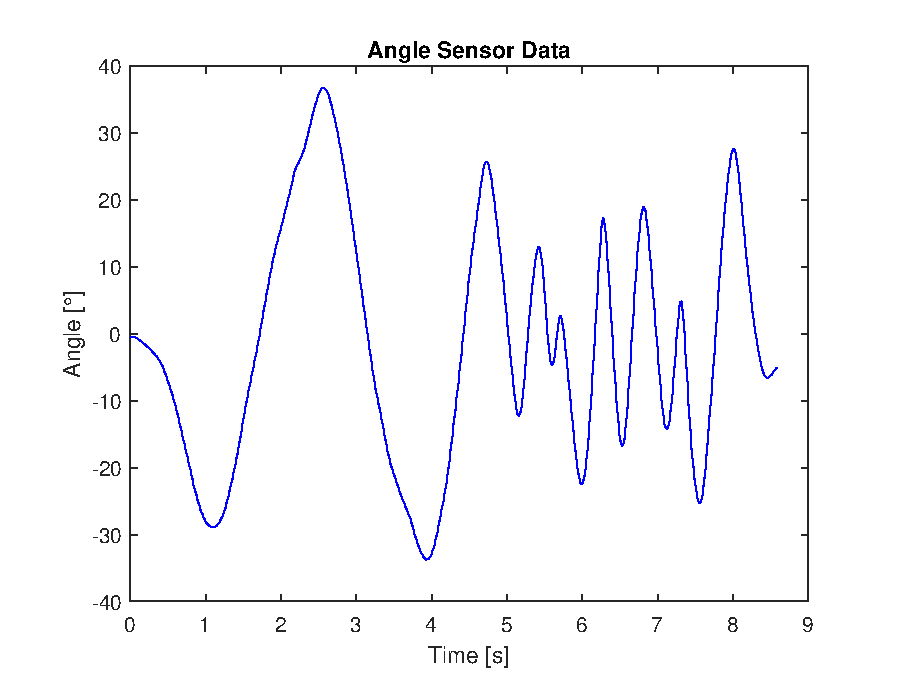
\includegraphics[width=.9\linewidth]{figures/plot_angle.eps}
    \caption{Angle measurements from the IMU.}
    \label{fig:imu_angle}
\end{figure}

\noindent
The structure was then laid still while the angular velocity from the gyrometer was measured at 10 ms intervals. The results can be seen in Figure~\ref{fig:imu_gyro}.

\begin{figure}[H]
    \centering
    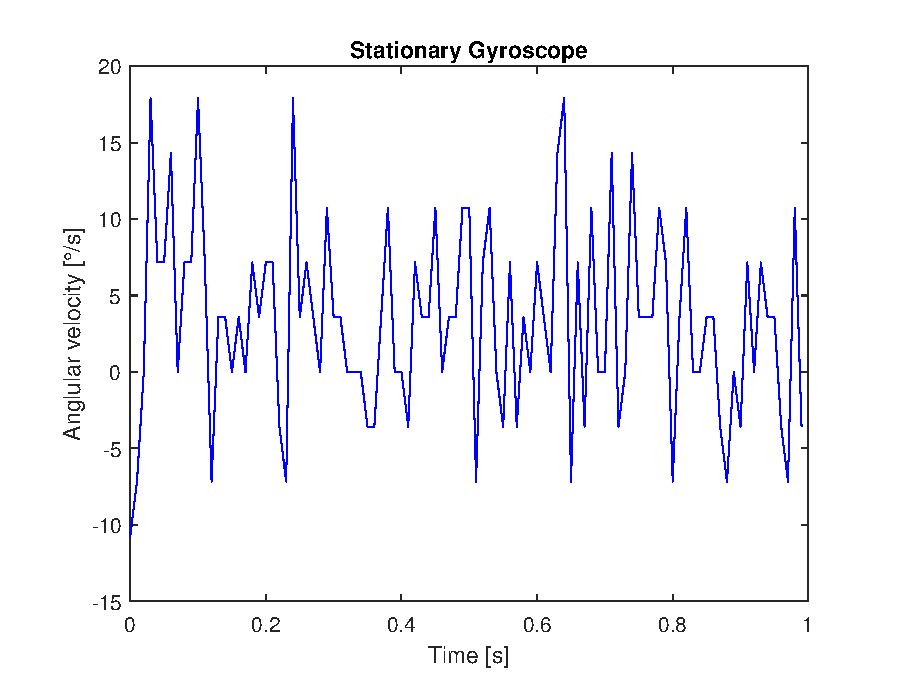
\includegraphics[width=.9\linewidth]{figures/plot_stationary.eps}
    \caption{Angular velocity measurements from the IMU.}
    \label{fig:imu_gyro}
\end{figure}

\subsection{Simulations}
The model in \eqref{eq:state-space} and \eqref{eq:ss-matrices} was simulated using both a PID controller and a LQG controller. The simulation results can be seen in Figure~\ref{fig:PIDGraph} and Figure~\ref{fig:LQGGraph}. For both simulations, a sample time of 15 ms and a pulse disturbance of $0.5\degree$ was used.
\\\\
The parameter settings for the discrete PID controller can be seen in Table~\ref{table:PIDParameters}.

\begin{table}[H]
    \centering
    \begin{tabular}{cc}\toprule
     Parameter  & Value \\\midrule
     $K_{P}$      & 3\\
     $K_{I}$      & 1\\
     $K_{D}$      & 0.3\\\bottomrule
    \end{tabular}
    \caption{The chosen PID parameters.}
    \label{table:PIDParameters}
\end{table}

\noindent
The optimal gain matrices $K$ and $L$ were calculated as

\begin{equation}
    \begin{gathered}
        K =
        \begin{bmatrix}
            6.0497 & 0.7365 & 0.0611
        \end{bmatrix}
        ,\\
        L = 
        \begin{bmatrix}
            1       & 0\\
            14.0934 & 0.0825\\
            0.8845  & 0.0048\\
        \end{bmatrix}
        .
    \end{gathered}
\end{equation}

\begin{figure}[h]
    \centering
    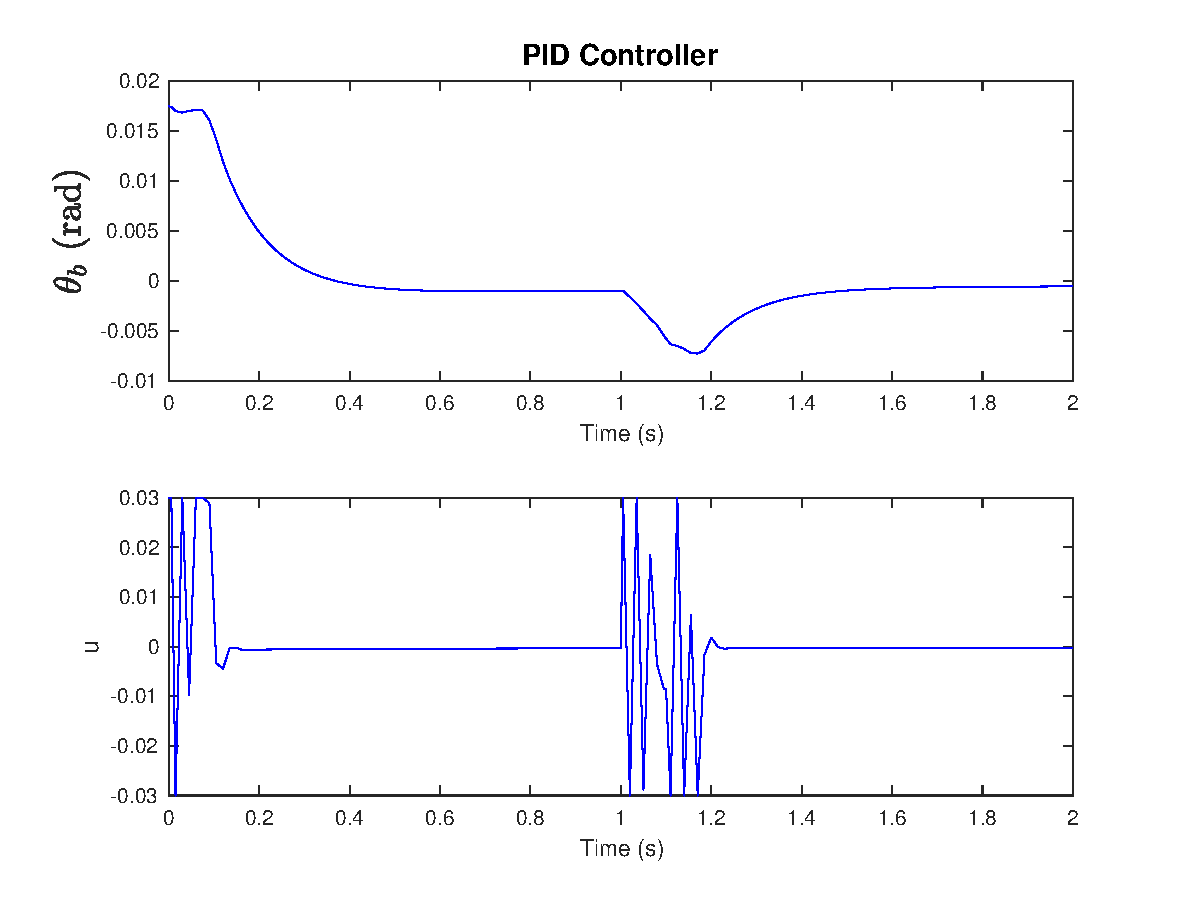
\includegraphics[width=\linewidth]{figures/PID.eps}
    \caption{Simulation of the single axis setup with a disturbance, using the PID controller.}
    \label{fig:PIDGraph}
\end{figure}

\begin{figure}[h]
    \centering
    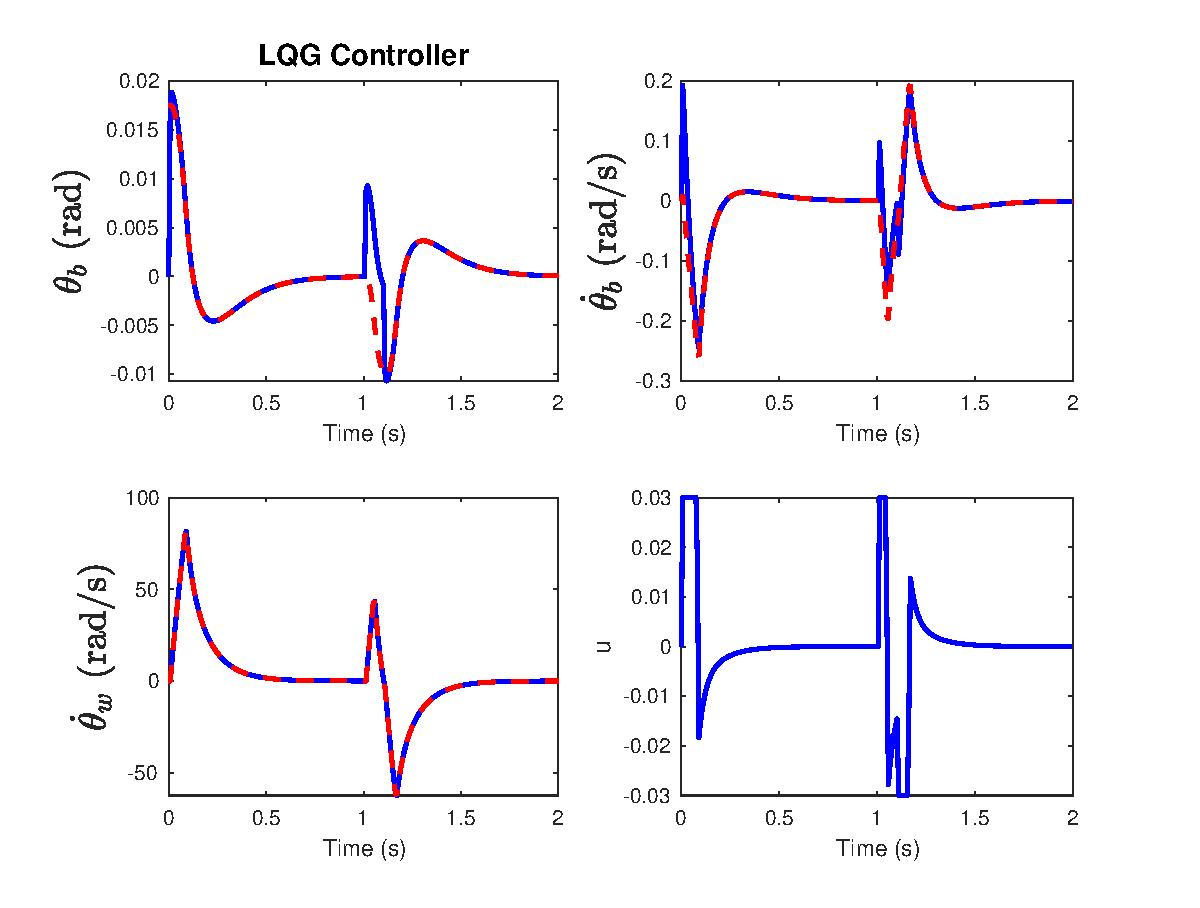
\includegraphics[width=\linewidth]{figures/LQG.eps}
    \caption{Simulation of the single axis setup with a disturbance, using the LQG controller. The blue line represents the estimated values and the red dashed line represents the values calculated from the state-space model.}
    \label{fig:LQGGraph}
\end{figure}

\noindent
While experimenting with different parameter settings for the simulation, we observed that some had a larger effect on the system than others. By changing the parameters in the PID simulation, with different factors, the parameters importance could be observed. The observation was based on how high, or low, of a factor a parameter could handle, before the system achieved instability. Sampling time, maximum torque and length to center of mass had the largest effect. This was followed by the mass of the frame and the radius of the wheel. In contrast, the system was still stable with a high friction coefficient and a low mass of the wheel. This qualitative observation is summarized in Table~\ref{table:ParamSig}.

\begin{table}[H]
    \centering
    \begin{tabular}{ccc}\toprule
            Parameter  & Factor & Importance \\\midrule
            $\Delta t$        & 1.2         & Very high\\
            $T_{\text{max}}$  & $2.7^{-1}$  & High\\
            $l$               & 2.8         & High\\
            $m_b$             & 4.5         & Medium\\
            $r_{w}$           & $4.5^{-1}$  & Medium\\
            $m_{w}$           & $< 20^{-1}$ & Low\\
            $C_{w}$           &  40         & Low\\\bottomrule
    \end{tabular}
    \caption{Parameters and their observed importance.}
    \label{table:ParamSig}
\end{table}

\subsection{The physical setup}
The discretized controller from \eqref{eq:PIDdisc} was implemented with a sample time of 10 ms with the original DC motors given to us. The motor was eventually swapped out to the new one\cite{motor-datasheet}. After this, testing could begin again. This time the motor feedback from \eqref{eq:PIDCdisc} was also implemented. Experimenting with PD-control and positive values of $K_C$ seemed promising but balancing still proved difficult. In a last ditch effort a new design for the pendulum body was made. The improved structure can be seen in Figure~\ref{fig:SingleAxisV2}.
\\\\
After some inspiration from\cite{LEGO-video} the controller now made use of integral action with a positive $K_I$ as well as reference adjustment according to \eqref{eq:ref-adjustment}. $K_C$ was now chosen to be negative and relatively small. The idea was to slow down the wheel over time when balancing. After some tuning stable balancing was finally achieved with the following control parameters:

\begin{equation}
    \begin{gathered}
        K_P = 50, \ \ K_I = 150, \ \ K_D = 2.5, \ \ K_C=-0.2, \\
        I_{\text{max}} = 127, \ \ \Delta \theta = 0.004.
    \end{gathered}
\end{equation}

\noindent
Note that the control signal ranges between $\pm255$ (where 255 is simply the max speed of the motor) and the output signal is measured in degrees. The parameter $\Delta \theta$ is also in degrees. In the code implementation, $\Delta t$ was also baked into the constants to reduce the amount of calculations. In Figure~\ref{fig:physical-balance} we can see roughly 15 seconds of balance using the control parameters above. The sensor readings shown are spaced 50 ms apart, but the controller still acted at the usual 10 ms intervals.

\begin{figure}[H]
    \centering
    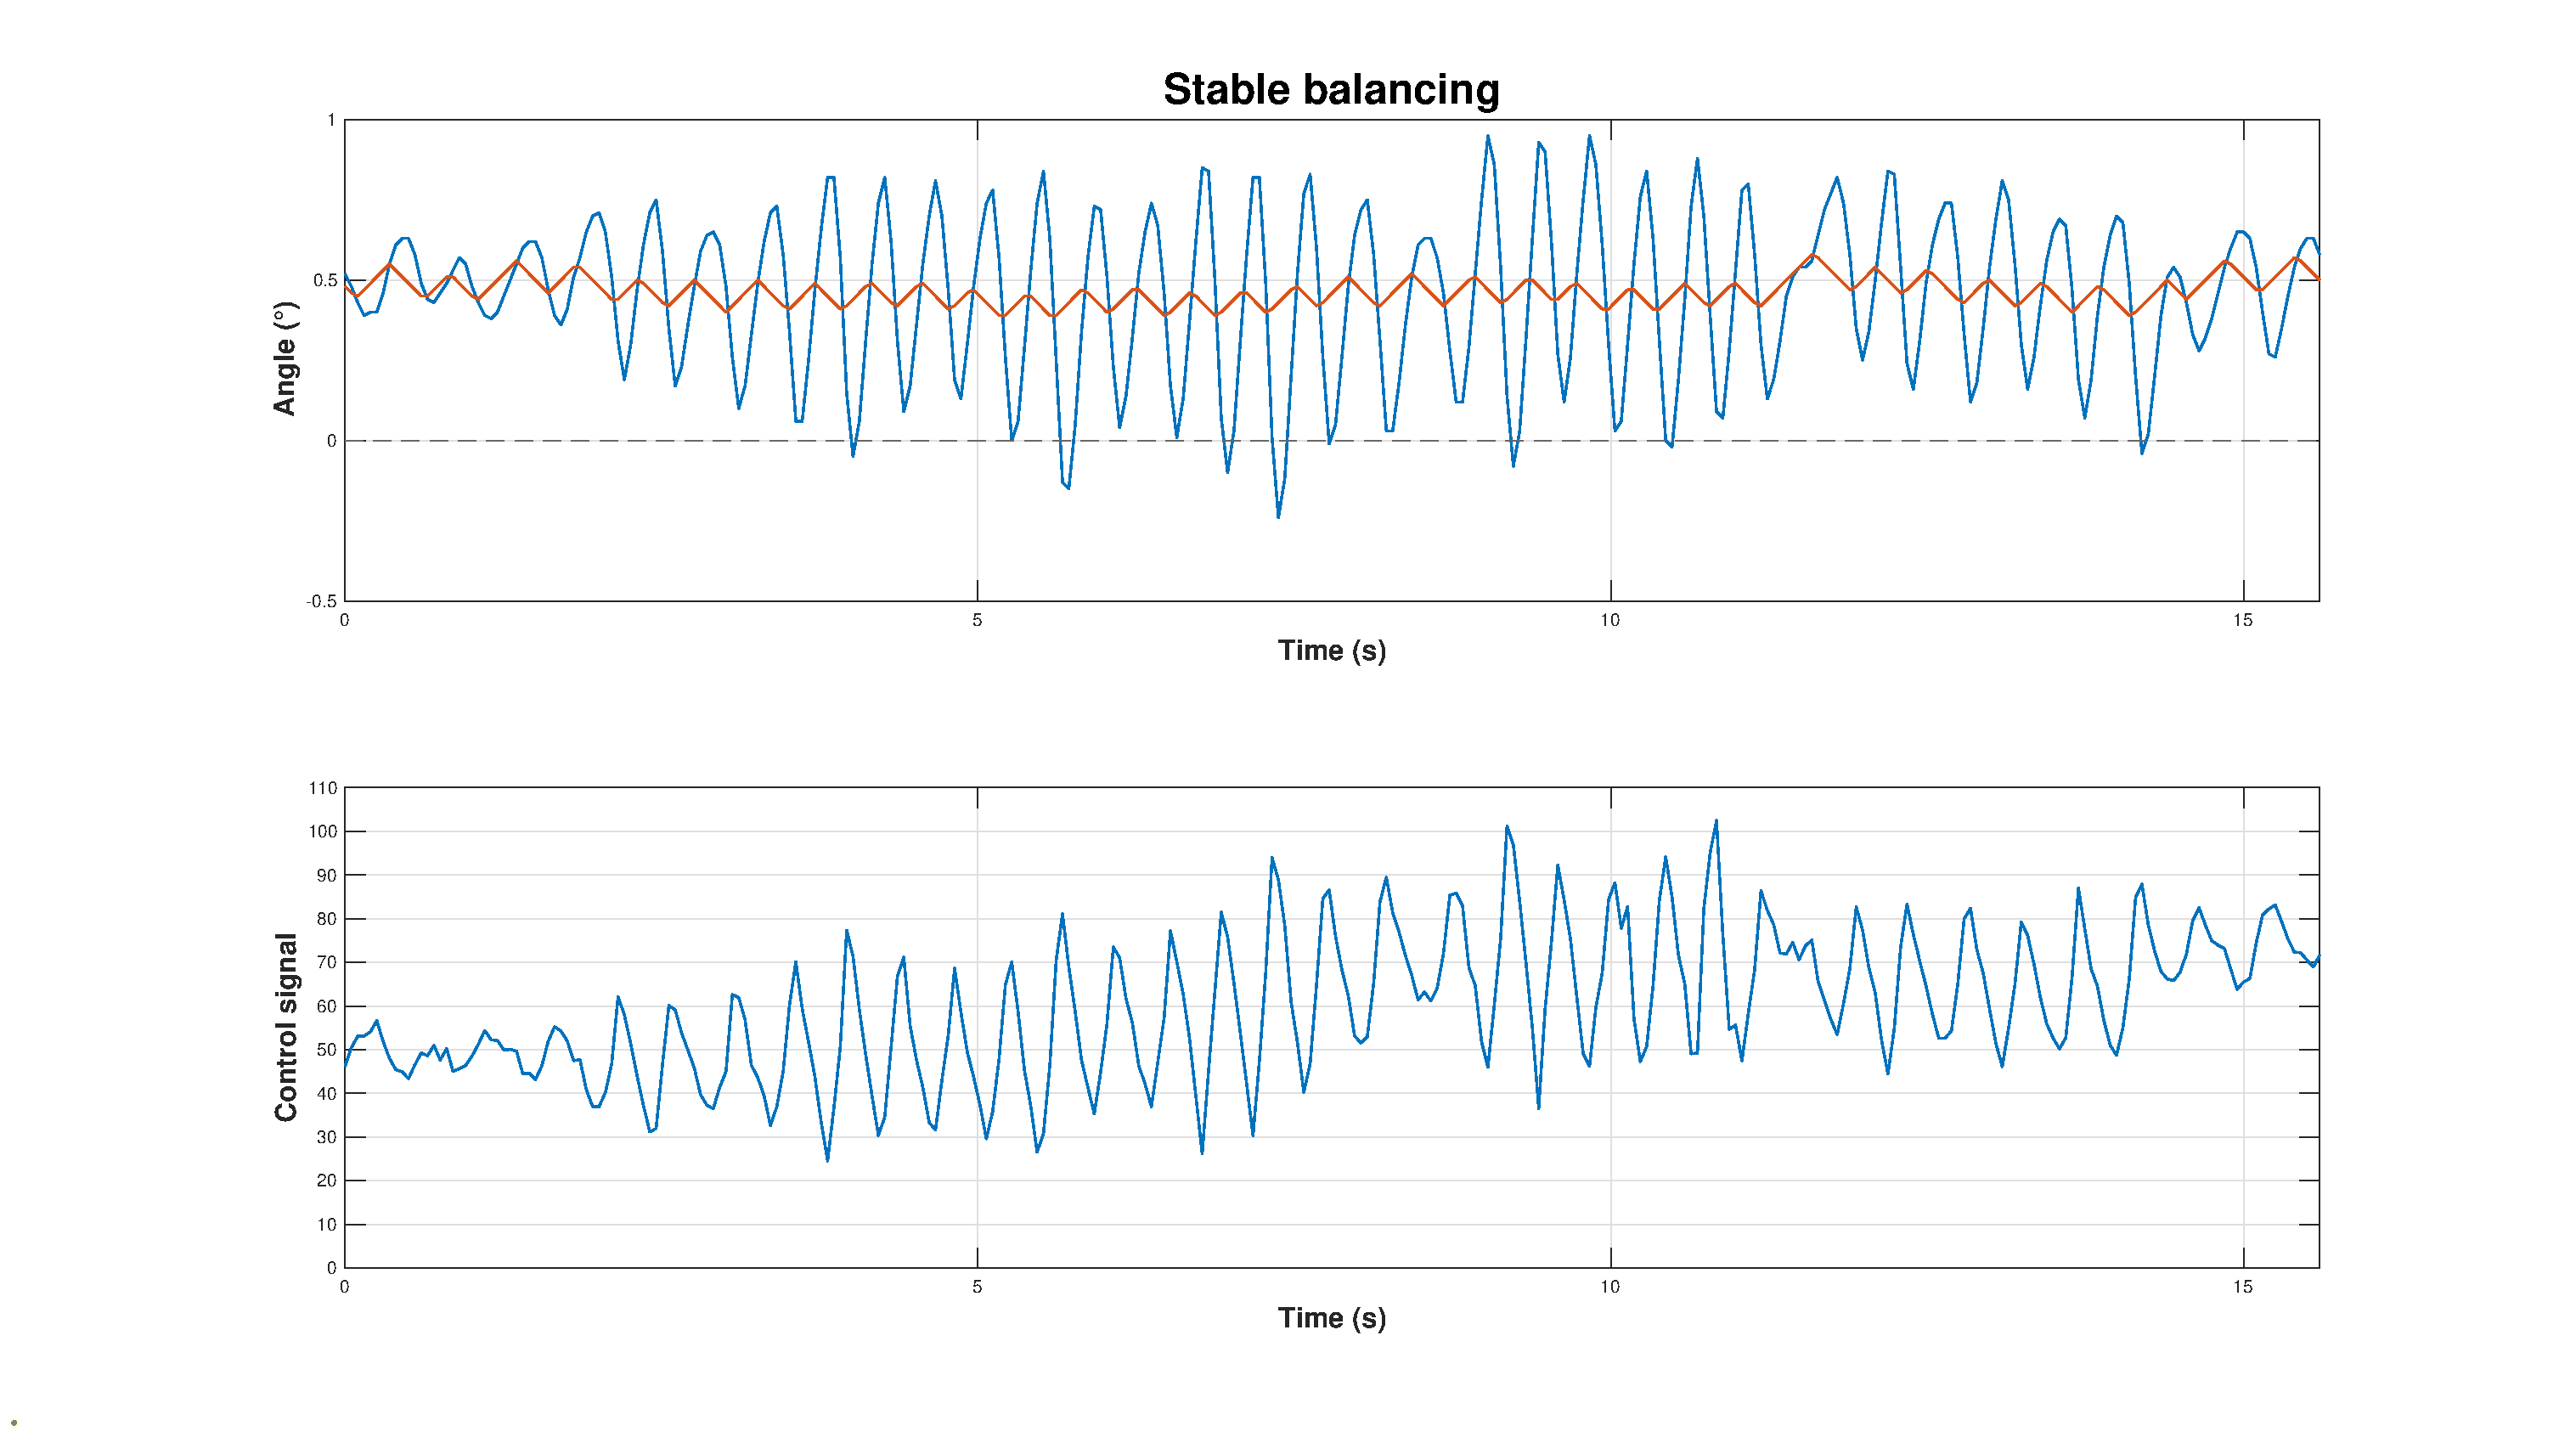
\includegraphics[width=1.2\linewidth, center]{figures/balance_with_u.eps}
    \caption{Top graph: the measured angle $\theta_b$ is in blue and $r$ is in orange. Bottom graph is the control signal.}
    \label{fig:physical-balance}
\end{figure}

\noindent
There are some key takeaways from this graph. Firstly, The structure is not balancing around $0\degree$. Instead, the reference is oscillating slightly around $0.46\degree$. The standard deviation in error over this period was $\sigma_e = 0.24\degree$. Secondly, the control signal is also oscillating around a positive, non-zero speed.
\\\\
Note that these 15 seconds were an excerpt from a longer period of balancing. In reality, the structure could balance for several minutes. The longest measured time balancing was just shy of 37 minutes. It could also handle small disturbances such as shaking the table and gently pushing the structure.

\subsection{The cube}
The physical model can be seen in Figure~\ref{fig:AssembledCube}. The printed parts, structural screws and nuts had a total mass of 587 grams. The scale that was used had an upper limit of 1 kg, which the cube exceeded with the rest of the internal components assembled.

\begin{figure}[H]
    \centering
    \begin{subfigure}[h]{0.2\textwidth}
        \centering
        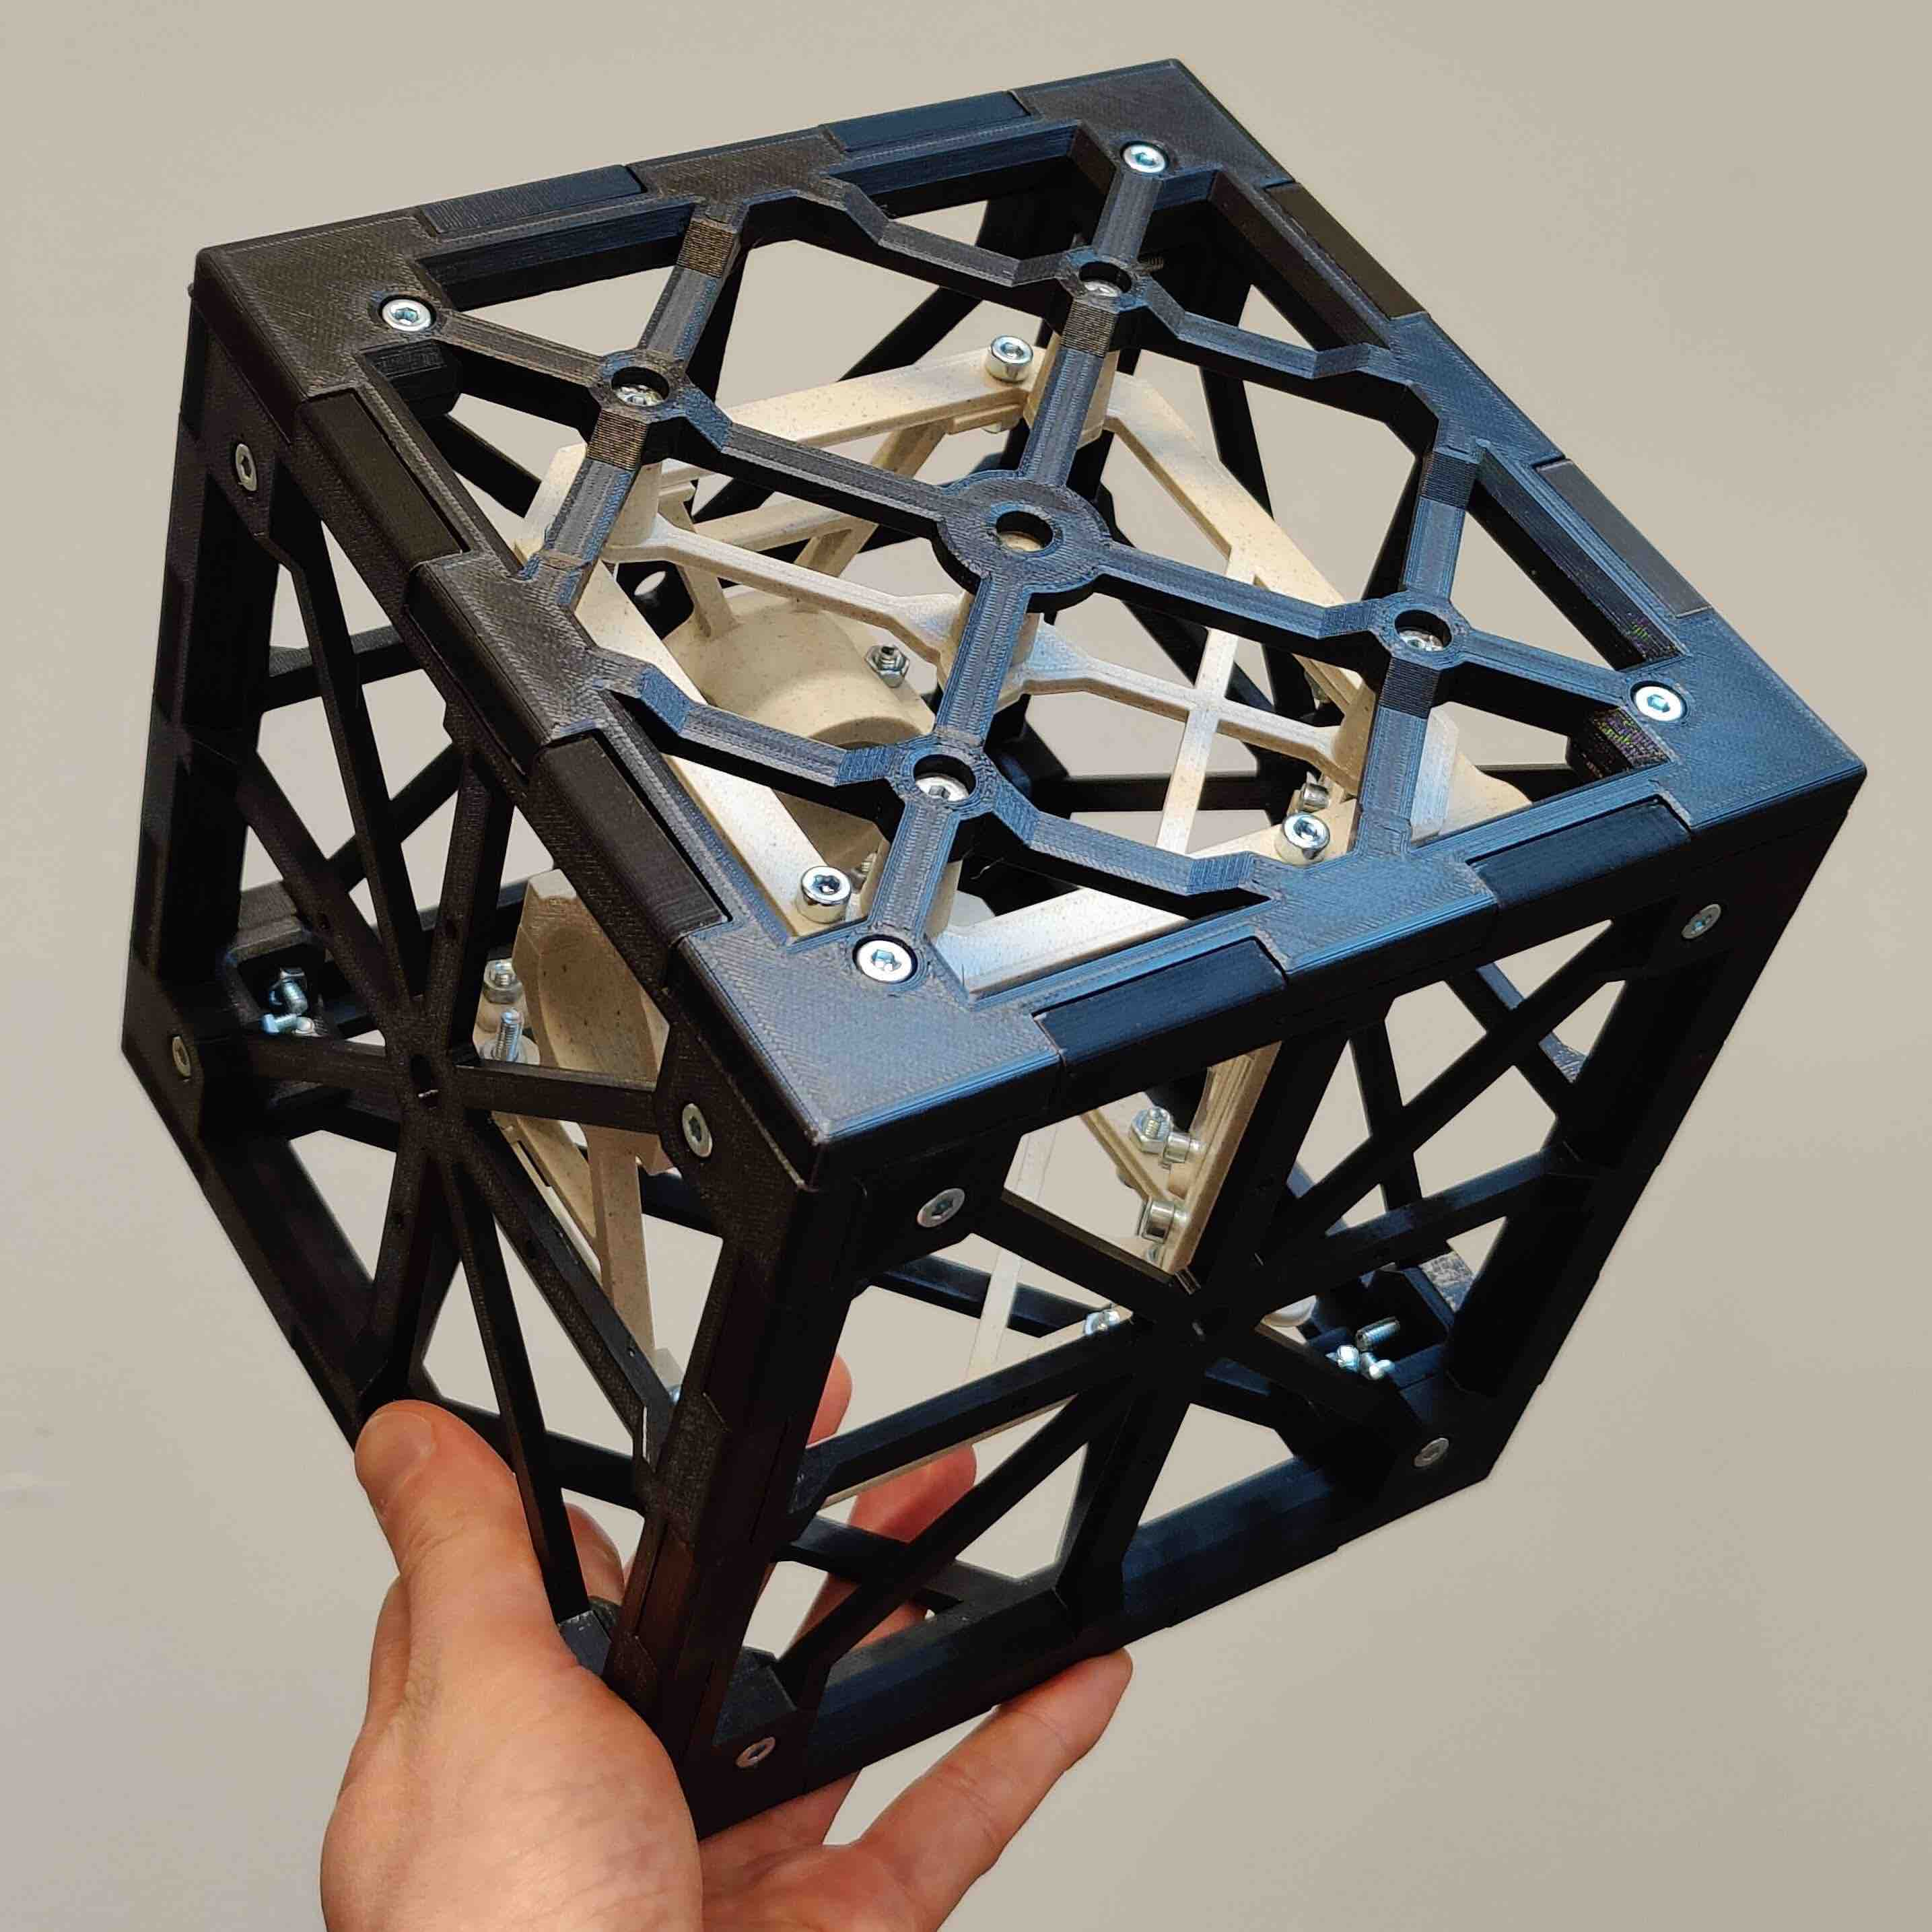
\includegraphics[width=\textwidth]{figures/CubeNoComponents.jpg}
        %\caption{Without electrical components}
        \label{fig:cubeNoComp}
    \end{subfigure}
    \begin{subfigure}[h]{0.2\textwidth}
        \centering
        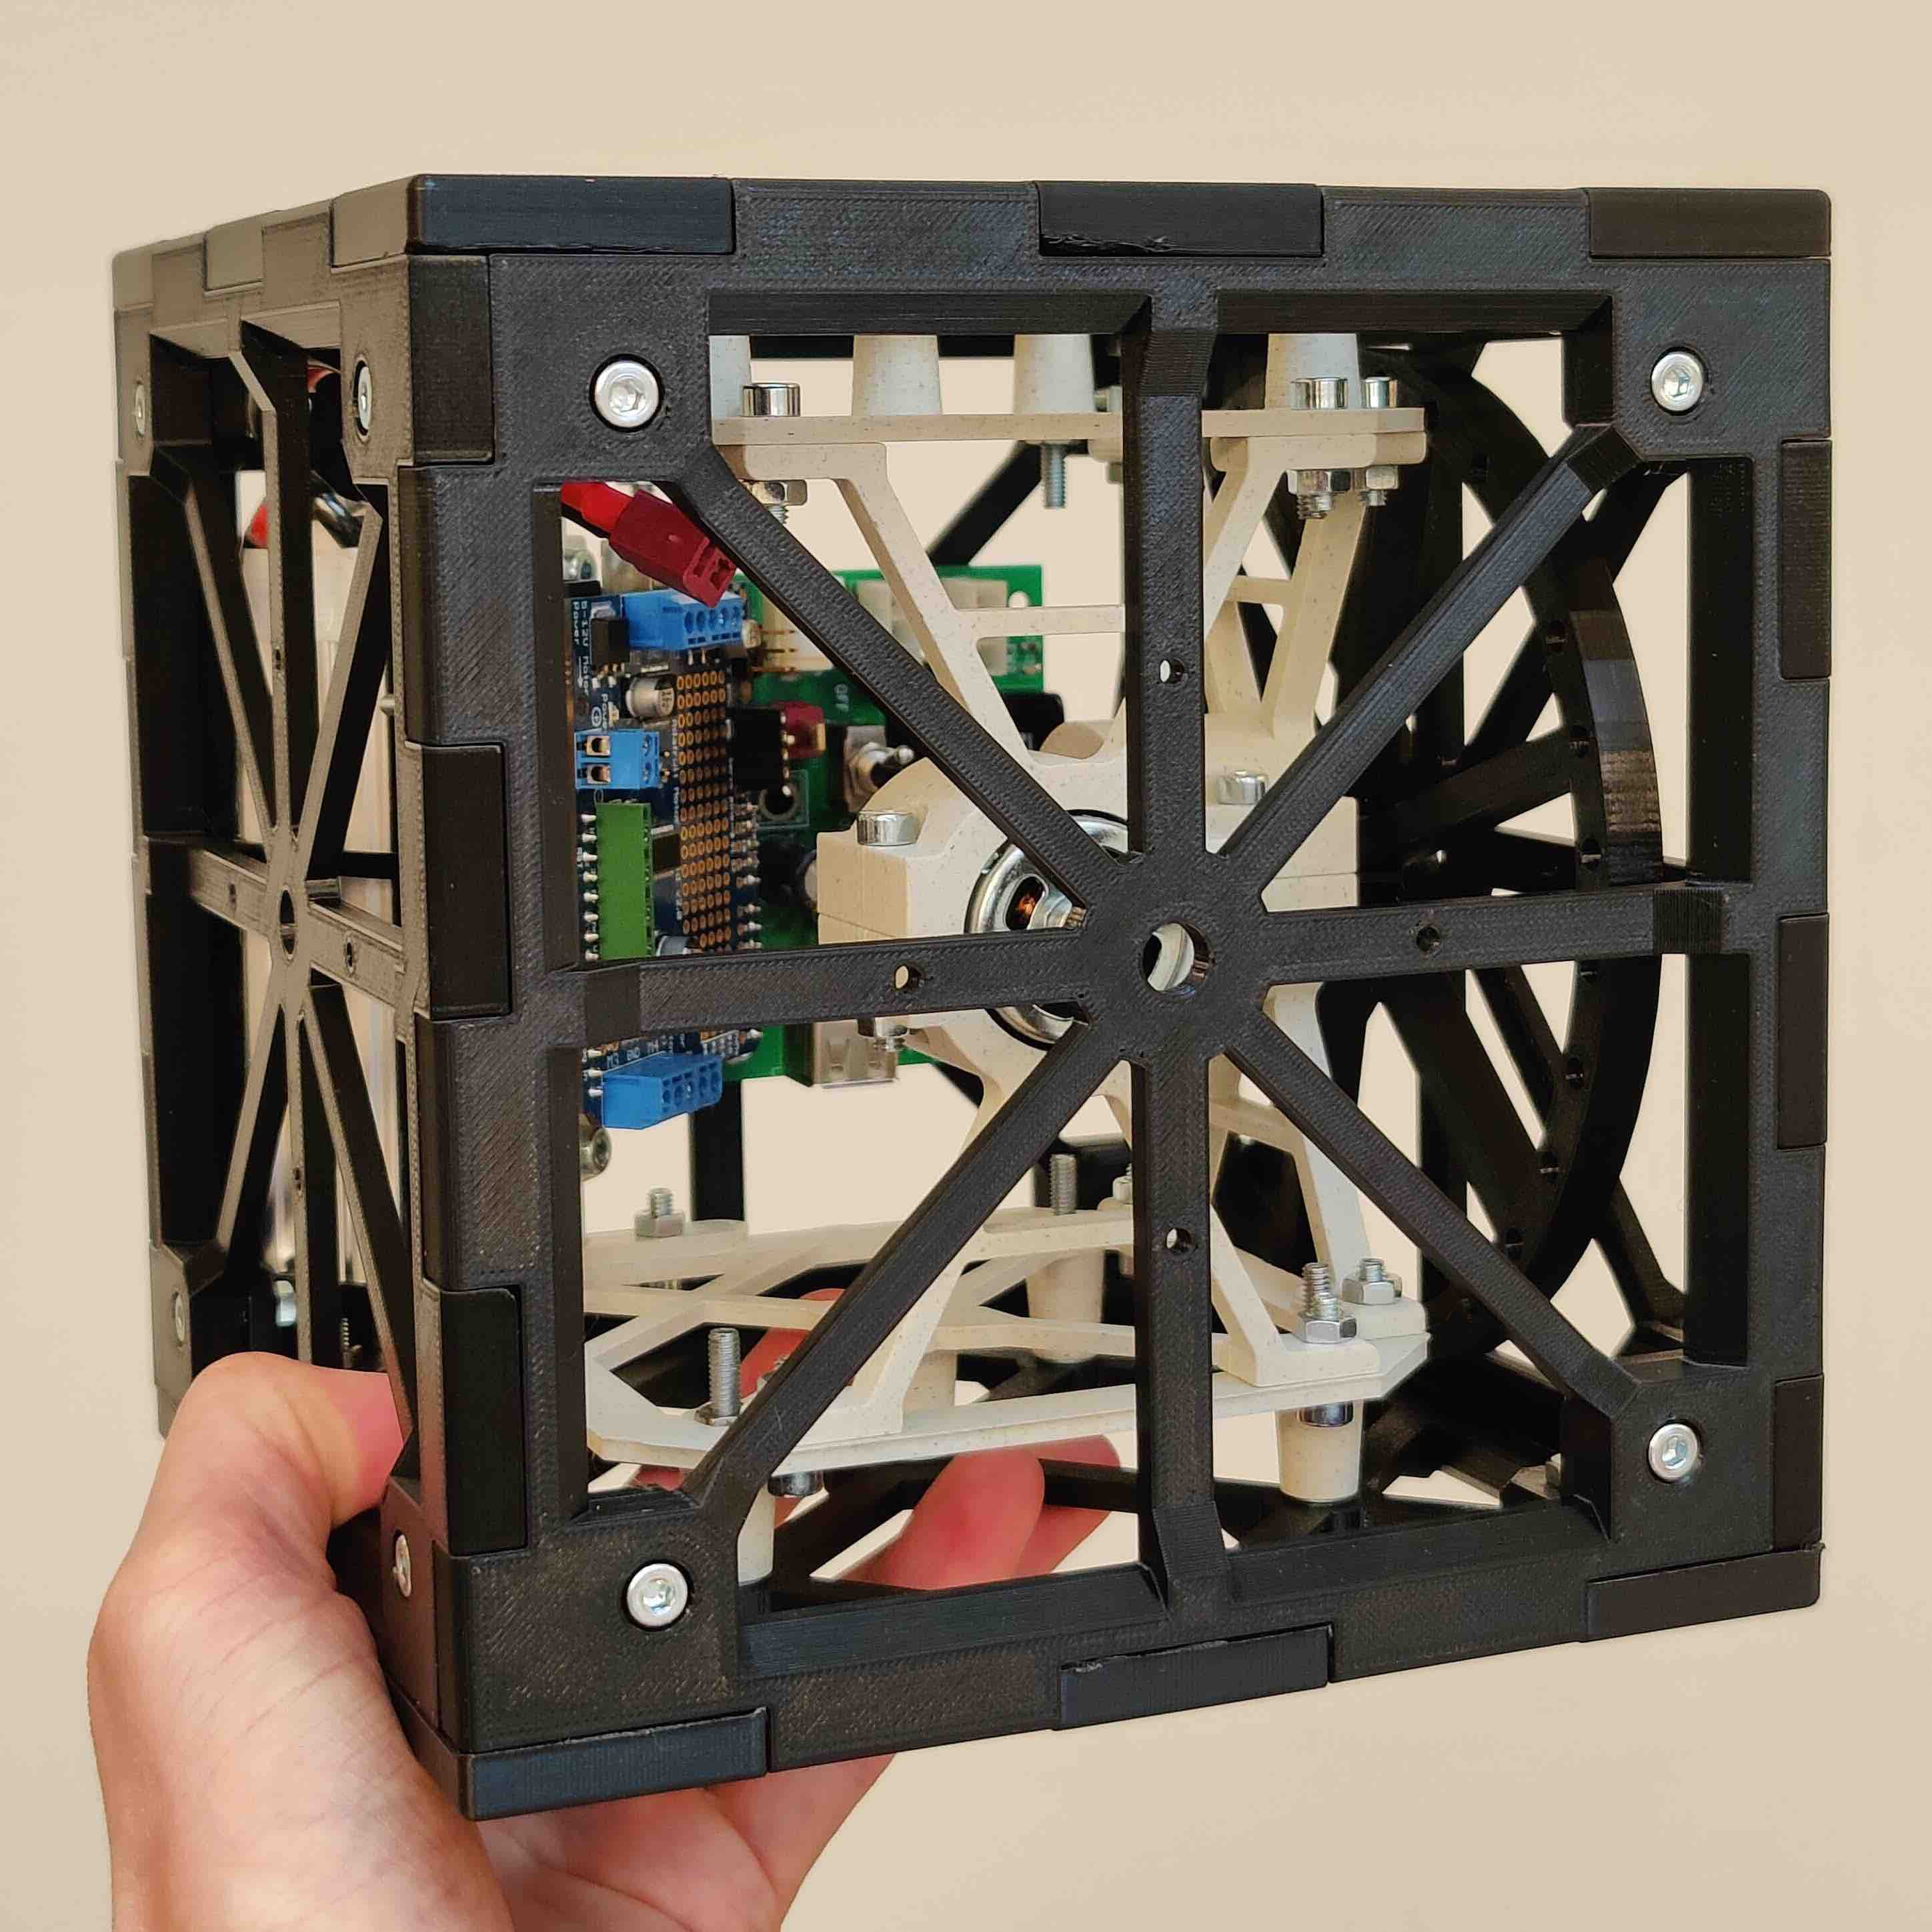
\includegraphics[width=\textwidth]{figures/CubeWithComponents.jpg}
        %\caption{With electrical components}
        \label{fig:cubeWith}
    \end{subfigure}
    \caption{The printed cube with and without components}
    \label{fig:AssembledCube}
\end{figure}
